%        File: arfc-beamer.tex
%     Created: Sun May 5 10:00 PM 2013 C
%


%\documentclass[11pt,handout]{beamer}
\documentclass[9pt]{beamer}
\usetheme[white]{Illinois}
%\title[short title]{long title}
\title[Impact of $^{135}$Xe on Load Following TAP MSR]{The Impact of 
Xenon-135 on Load Following Transatomic Power Molten 
Salt Reactor}
%\subtitle[short subtitle]{long subtitle}
%\subtitle[Short SubTitle]{Mostly Kittens}
%\author[short name]{long name}
\author[Andrei Rykhlevskii]{Andrei Rykhlevskii, Daniel O'Grady, Tomasz 
Kozlowski, Kathryn Huff\\Advanced Reactors and Fuel Cycles Group}
%\date[short date]{long date}
\date[11.19.2019]{November 19, 2019}
%\institution[short name]{long name}
\institute[UIUC]{University of Illinois at Urbana-Champaign}


\usepackage{lmodern}

%\usepackage{bbding}
\usepackage{tikz}
\usepackage{amsfonts}
\usepackage{amsmath}
\usepackage{caption}  % allows center figures caption
\usepackage{xspace}
\usepackage{notoccite}
\usepackage{graphicx}
\usepackage{animate}
\usepackage{subfigure}
\usepackage{booktabs} % nice rules for tables
\usepackage{microtype} % if using PDF
\usepackage{bigints}
\usepackage[absolute,overlay]{textpos}
%\usepackage{minted}
\usepackage{xcolor}
\usepackage{soul}
\newcommand{\hlc}[2][yellow]{{%
    \colorlet{foo}{#1}%
    \sethlcolor{foo}\hl{#2}}%
}
\newcommand{\units}[1] {\:\text{#1}}%
\newcommand{\SN}{S$_N$}%{S$_\text{N}$}%{$S_N$}%
\DeclareMathOperator{\erf}{erf}
%I need some complimentary error funcitons... 
\DeclareMathOperator{\erfc}{erfc}
%page numbers
\setbeamertemplate{page number in head/foot}[appendixframenumber]
\setbeamertemplate{caption}[numbered]
%Those icons in the references are terrible looking
\setbeamertemplate{bibliography item}[text]
\setbeamercovered{dynamic}
%%%% Acronym support

\usepackage[acronym,toc]{glossaries}
%\newacronym{<++>}{<++>}{<++>}
\newacronym[longplural={metric tons of heavy metal}]{MTHM}{MTHM}{metric ton of heavy metal}
\newacronym{ABM}{ABM}{agent-based modeling}
\newacronym{ACDIS}{ACDIS}{Program in Arms Control \& Domestic and International Security}
\newacronym{AHTR}{AHTR}{Advanced High Temperature Reactor}
\newacronym{ANDRA}{ANDRA}{Agence Nationale pour la gestion des D\'echets RAdioactifs, the French National Agency for Radioactive Waste Management}
\newacronym{ANL}{ANL}{Argonne National Laboratory}
\newacronym{ANS}{ANS}{American Nuclear Society}
\newacronym{API}{API}{application programming interface}
\newacronym{ARE}{ARE}{Aircraft Reactor Experiment}
\newacronym{ARFC}{ARFC}{Advanced Reactors and Fuel Cycles}
\newacronym{ASME}{ASME}{American Society of Mechanical Engineers}
\newacronym{ATWS}{ATWS}{Anticipated Transient Without Scram}
\newacronym{BOL}{BOL}{Beginning of Life}
\newacronym{BDBE}{BDBE}{Beyond Design Basis Event}
\newacronym{BIDS}{BIDS}{Berkeley Institute for Data Science}
\newacronym{BWR}{BWR}{Boiling Water Reactor}
\newacronym{CAFCA}{CAFCA}{ Code for Advanced Fuel Cycles Assessment }
\newacronym{CDTN}{CDTN}{Centro de Desenvolvimento da Tecnologia Nuclear}
\newacronym{CFD}{CFD}{Computational Fluid Dynamics}
\newacronym{CEA}{CEA}{Commissariat \`a l'\'Energie Atomique et aux \'Energies Alternatives}
\newacronym{CI}{CI}{continuous integration}
\newacronym{CNEN}{CNEN}{Comiss\~{a}o Nacional de Energia Nuclear}
\newacronym{CNERG}{CNERG}{Computational Nuclear Engineering Research Group}
\newacronym{COSI}{COSI}{Commelini-Sicard}
\newacronym{COTS}{COTS}{commercial, off-the-shelf}
\newacronym{CSNF}{CSNF}{commercial spent nuclear fuel}
\newacronym{CTAH}{CTAHs}{Coiled Tube Air Heaters}
\newacronym{CUBIT}{CUBIT}{CUBIT Geometry and Mesh Generation Toolkit}
\newacronym{CURIE}{CURIE}{Centralized Used Fuel Resource for Information Exchange}
\newacronym{CR}{CR}{conversion ratio}
\newacronym{DAG}{DAG}{directed acyclic graph}
\newacronym{DANESS}{DANESS}{Dynamic Analysis of Nuclear Energy System Strategies}
\newacronym{DBE}{DBE}{Design Basis Event}
\newacronym{DESAE}{DESAE}{Dynamic Analysis of Nuclear Energy Systems Strategies}
\newacronym{DHS}{DHS}{Department of Homeland Security}
\newacronym{DOE}{DOE}{Department of Energy}
\newacronym{DRACS}{DRACS}{Direct Reactor Auxiliary Cooling System}
\newacronym{DRE}{DRE}{dynamic resource exchange}
\newacronym{DSNF}{DSNF}{DOE spent nuclear fuel}
\newacronym{DYMOND}{DYMOND}{Dynamic Model of Nuclear Development }
\newacronym{EBS}{EBS}{Engineered Barrier System}
\newacronym{EDF}{EDF}{Électricité de France}
\newacronym{EDZ}{EDZ}{Excavation Disturbed Zone}
\newacronym{EOL}{EOL}{End of Life}
\newacronym{EIA}{EIA}{U.S. Energy Information Administration}
\newacronym{EPA}{EPA}{Environmental Protection Agency}
\newacronym{EPR}{EPR}{European Pressurized Reactors}
\newacronym{EP}{EP}{Engineering Physics}
\newacronym{EU}{EU}{European Union}
\newacronym{FCO}{FCO}{Fuel Cycle Options}
\newacronym{FCT}{FCT}{Fuel Cycle Technology}
\newacronym{FEHM}{FEHM}{Finite Element Heat and Mass Transfer}
\newacronym{FEPs}{FEPs}{Features, Events, and Processes}
\newacronym{FHR}{FHR}{Fluoride-Salt-Cooled High-Temperature Reactor}
\newacronym{FLiBe}{FLiBe}{Fluoride-Lithium-Beryllium}
\newacronym{FP}{FP}{Fission Product}
\newacronym{GDSE}{GDSE}{Generic Disposal System Environment}
\newacronym{GDSM}{GDSM}{Generic Disposal System Model}
\newacronym{GENIUSv1}{GENIUSv1}{Global Evaluation of Nuclear Infrastructure Utilization Scenarios, Version 1}
\newacronym{GENIUSv2}{GENIUSv2}{Global Evaluation of Nuclear Infrastructure Utilization Scenarios, Version 2}
\newacronym{GENIUS}{GENIUS}{Global Evaluation of Nuclear Infrastructure Utilization Scenarios}
\newacronym{GPAM}{GPAM}{Generic Performance Assessment Model}
\newacronym{GRSAC}{GRSAC}{Graphite Reactor Severe Accident Code}
\newacronym{GUI}{GUI}{graphical user interface}
\newacronym{HLW}{HLW}{high level waste}
\newacronym{HPC}{HPC}{high-performance computing}
\newacronym{HTC}{HTC}{high-throughput computing}
\newacronym{HTGR}{HTGR}{High Temperature Gas-Cooled Reactor}
\newacronym{IAEA}{IAEA}{International Atomic Energy Agency}
\newacronym{IEMA}{IEMA}{Illinois Emergency Mangament Agency}
\newacronym{IHLRWM}{IHLRWM}{International High Level Radioactive Waste Management}
\newacronym{INL}{INL}{Idaho National Laboratory}
\newacronym{IPRR1}{IRP-R1}{Instituto de Pesquisas Radioativas Reator 1}
\newacronym{IRP}{IRP}{Integrated Research Project}
\newacronym{ISFSI}{ISFSI}{Independent Spent Fuel Storage Installation}
\newacronym{ISRG}{ISRG}{Independent Student Research Group}
\newacronym{JFNK}{JFNK}{Jacobian-Free Newton Krylov}
\newacronym{LANL}{LANL}{Los Alamos National Laboratory}
\newacronym{LBNL}{LBNL}{Lawrence Berkeley National Laboratory}
\newacronym{LCOE}{LCOE}{levelized cost of electricity}
\newacronym{LEU}{LEU}{low-enriched uranium}
\newacronym{LDRD}{LDRD}{laboratory directed research and development}
\newacronym{LFR}{LFR}{Lead-Cooled Fast Reactor}
\newacronym{LLNL}{LLNL}{Lawrence Livermore National Laboratory}
\newacronym{LMFBR}{LMFBR}{Liquid Metal Fast Breeder Reactor}
\newacronym{LOFC}{LOFC}{Loss of Forced Cooling}
\newacronym{LOHS}{LOHS}{Loss of Heat Sink}
\newacronym{LOLA}{LOLA}{Loss of Large Area}
\newacronym{LP}{LP}{linear program}
\newacronym{LWR}{LWR}{Light Water Reactor}
\newacronym{MAGNOX}{MAGNOX}{Magnesium Alloy Graphie Moderated Gas Cooled Uranium Oxide Reactor}
\newacronym{MA}{MA}{minor actinide}
\newacronym{MCNP}{MCNP}{Monte Carlo N-Particle code}
\newacronym{MILP}{MILP}{mixed-integer linear program}
\newacronym{MIT}{MIT}{the Massachusetts Institute of Technology}
\newacronym{MOAB}{MOAB}{Mesh-Oriented datABase}
\newacronym{MOOSE}{MOOSE}{Multiphysics Object-Oriented Simulation Environment}
\newacronym{MOSART}{MOSART}{Molten Salt Actinide Recycler and Transmuter}
\newacronym{MOX}{MOX}{mixed oxide}
\newacronym{MPI}{MPI}{Message Passing Interface}
\newacronym{MSBR}{MSBR}{Molten Salt Breeder Reactor}
\newacronym{MSFR}{MSFR}{Molten Salt Fast Reactor}
\newacronym{MSRE}{MSRE}{Molten Salt Reactor Experiment}
\newacronym{MSR}{MSR}{Molten Salt Reactor}
\newacronym{NAGRA}{NAGRA}{National Cooperative for the Disposal of Radioactive Waste}
\newacronym{NEAMS}{NEAMS}{Nuclear Engineering Advanced Modeling and Simulation}
\newacronym{NEUP}{NEUP}{Nuclear Energy University Programs}
\newacronym{NFCSim}{NFCSim}{Nuclear Fuel Cycle Simulator}
\newacronym{NGNP}{NGNP}{Next Generation Nuclear Plant}
\newacronym{NMWPC}{NMWPC}{Nuclear MW Per Capita}
\newacronym{NNSA}{NNSA}{National Nuclear Security Administration}
\newacronym{NPP}{NPP}{Nuclear Power Plant}
\newacronym{NPRE}{NPRE}{Department of Nuclear, Plasma, and Radiological Engineering}
\newacronym{NQA1}{NQA-1}{Nuclear Quality Assurance - 1}
\newacronym{NRC}{NRC}{Nuclear Regulatory Commission}
\newacronym{NSF}{NSF}{National Science Foundation}
\newacronym{NSSC}{NSSC}{Nuclear Science and Security Consortium}
\newacronym{NUWASTE}{NUWASTE}{Nuclear Waste Assessment System for Technical Evaluation}
\newacronym{NWF}{NWF}{Nuclear Waste Fund}
\newacronym{NWTRB}{NWTRB}{Nuclear Waste Technical Review Board}
\newacronym{OCRWM}{OCRWM}{Office of Civilian Radioactive Waste Management}
\newacronym{OOP}{OOP}{Object-Orienting Programming}
\newacronym{ORION}{ORION}{ORION}
\newacronym{ORNL}{ORNL}{Oak Ridge National Laboratory}
\newacronym{PARCS}{PARCS}{Purdue Advanced Reactor Core Simulator}
\newacronym{PBAHTR}{PB-AHTR}{Pebble Bed Advanced High Temperature Reactor}
\newacronym{PBFHR}{PB-FHR}{Pebble-Bed Fluoride-Salt-Cooled High-Temperature Reactor}
\newacronym{PEI}{PEI}{Peak Environmental Impact}
\newacronym{PH}{PRONGHORN}{PRONGHORN}
\newacronym{PRIS}{PRIS}{Power Reactor Information System}
\newacronym{PRKE}{PRKE}{Point Reactor Kinetics Equations}
\newacronym{PSPG}{PSPG}{Pressure-Stabilizing/Petrov-Galerkin}
\newacronym{PWAR}{PWAR}{Pratt and Whitney Aircraft Reactor}
\newacronym{PWR}{PWR}{Pressurized Water Reactor}
\newacronym{PyNE}{PyNE}{Python toolkit for Nuclear Engineering}
\newacronym{PyRK}{PyRK}{Python for Reactor Kinetics}
\newacronym{QA}{QA}{quality assurance}
\newacronym{RDD}{RD\&D}{Research Development and Demonstration}
\newacronym{RD}{R\&D}{Research and Development}
\newacronym{REE}{REE}{rare earth element}
\newacronym{RELAP}{RELAP}{Reactor Excursion and Leak Analysis Program}
\newacronym{RIA}{RIA}{Reactivity Insertion Accident}
\newacronym{RIF}{RIF}{Region-Institution-Facility}
\newacronym{SFR}{SFR}{Sodium-Cooled Fast Reactor}
\newacronym{SINDAG}{SINDA{\textbackslash}G}{Systems Improved Numerical Differencing Analyzer $\backslash$ Gaski}
\newacronym{SKB}{SKB}{Svensk K\"{a}rnbr\"{a}nslehantering AB}
\newacronym{SNF}{SNF}{spent nuclear fuel}
\newacronym{SNL}{SNL}{Sandia National Laboratory}
\newacronym{STC}{STC}{specific temperature change}
\newacronym{SUPG}{SUPG}{Streamline-Upwind/Petrov-Galerkin}
\newacronym{SVF}{SVF}{salt volume fraction}
\newacronym{SWF}{SWF}{Separations and Waste Forms}
\newacronym{SWU}{SWU}{Separative Work Unit}
\newacronym{TAP}{TAP}{Transatomic Power}
\newacronym{TRIGA}{TRIGA}{Training Research Isotope General Atomic}
\newacronym{TRISO}{TRISO}{Tristructural Isotropic}
\newacronym{TSM}{TSM}{Total System Model}
\newacronym{TSPA}{TSPA}{Total System Performance Assessment for the Yucca Mountain License Application}
\newacronym{ThOX}{ThOX}{thorium oxide}
\newacronym{UFD}{UFD}{Used Fuel Disposition}
\newacronym{UML}{UML}{Unified Modeling Language}
\newacronym{UOX}{UOX}{uranium oxide}
\newacronym{UQ}{UQ}{uncertainty quantification}
\newacronym{US}{US}{United States}
\newacronym{UW}{UW}{University of Wisconsin}
\newacronym{VISION}{VISION}{the Verifiable Fuel Cycle Simulation Model}
\newacronym{VVER}{VVER}{Voda-Vodyanoi Energetichesky Reaktor (Russian Pressurized Water Reactor)}
\newacronym{VV}{V\&V}{verification and validation}
\newacronym{WIPP}{WIPP}{Waste Isolation Pilot Plant}
\newacronym{YMR}{YMR}{Yucca Mountain Repository Site}


\makeglossaries

%try to get rid of header on title page\dots
\makeatletter
    \newenvironment{withoutheadline}{
        \setbeamertemplate{headline}[default]
        \def\beamer@entrycode{\vspace*{-\headheight}}
    }{}
\makeatother

\begin{document}
%%%%%%%%%%%%%%%%%%%%%%%%%%%%%%%%%%%%%%%%%%%%%%%%%%%%%%%%%%%%%
%% From uw-beamer Here's a handy bit of code to place at 
%% the beginning of your presentation (after \begin{document}):
\newcommand*{\alphabet}{ABCDEFGHIJKLMNOPQRSTUVWXYZabcdefghijklmnopqrstuvwxyz}
\newlength{\highlightheight}
\newlength{\highlightdepth}
\newlength{\highlightmargin}
\setlength{\highlightmargin}{2pt}
\settoheight{\highlightheight}{\alphabet}
\settodepth{\highlightdepth}{\alphabet}
\addtolength{\highlightheight}{\highlightmargin}
\addtolength{\highlightdepth}{\highlightmargin}
\addtolength{\highlightheight}{\highlightdepth}
\newcommand*{\Highlight}{\rlap{\textcolor{HighlightBackground}{\rule[-\highlightdepth]{\linewidth}{\highlightheight}}}}
%%%%%%%%%%%%%%%%%%%%%%%%%%%%%%%%%%%%%%%%%%%%%%%%%%%%%%%%%%%%%
% Total slides number manual
%\def\inserttotalframenumber{41}
%%--------------------------------%%
\begin{withoutheadline}
\frame{
  \titlepage
}
\end{withoutheadline}

%%--------------------------------%%
\AtBeginSection[]{
\begin{frame}
  \frametitle{Outline}
  \tableofcontents[currentsection]
\end{frame}
}

\section{Introduction}
\begin{frame}
\frametitle{UIUC Project Overview}
        \begin{block}{ARPA-E MEITNER Award 1798-1576}
                \begin{itemize}
                        \item[\textbf{PI:}] Huff
                        \item[\textbf{Co-PIs:}] Brooks, Heuser, Kozlowski, Stubbins
                        \item[\textbf{Objective:}] This project will establish 
                                a xenon removal sparger design to enable load 
                                following in liquid-fueled MSRs at ramp rates 
                                comparable or superior to natural gas peaking 
                                generation, $\left(\frac{\pm 
                                10\%}{\mbox{minute}}\right)$.
                \end{itemize}
        \end{block}

        \begin{block}{Motivation}
\begin{itemize}
\item Load following Molten Salt Reactors are potentially transformative
\item But, feasible online xenon removal system designs are absent.
\end{itemize} 
  The UIUC project will unlock the benefits of MSRs by bounding these designs
        \begin{itemize}
                \item \textbf{via simulation of multiple physics}
                \begin{itemize}
                        \item fluid dynamics,
                        \item neutronics,
                        \item and fuel cycle dynamics.
                \end{itemize}
                \item \textbf{and with novel mass transport and sparging experiments.}
        \end{itemize}
        \end{block}
\end{frame}

\begin{frame}
\frametitle{UIUC Project Thrusts}
\begin{figure}
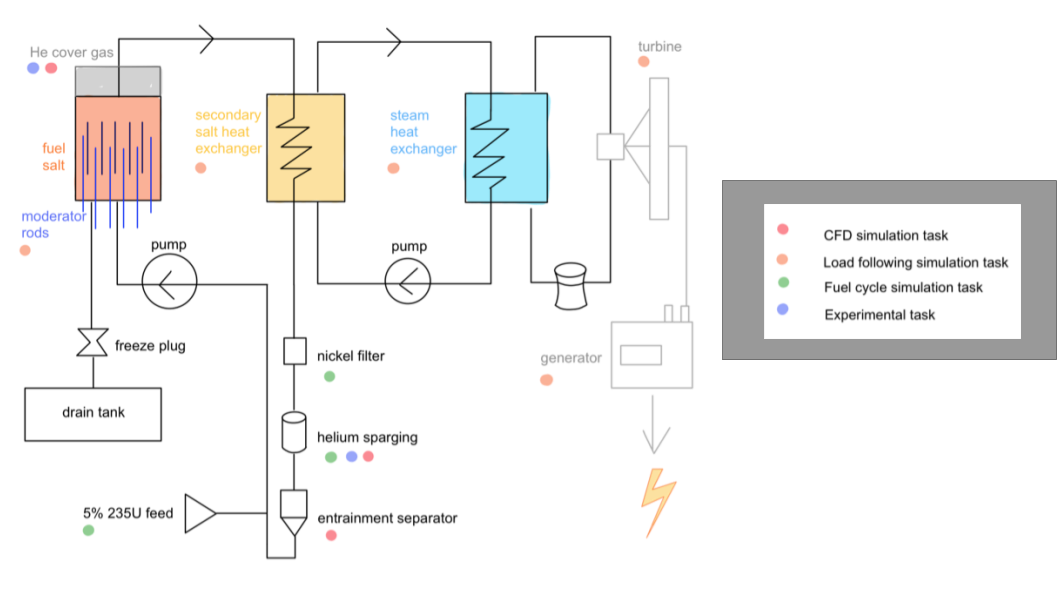
\includegraphics[width=\textwidth]{./images/system-diag.png}
        \caption{In \textbf{4 major thrusts} the project will establish a 
        feasible design for the sparging system, an overlooked MSR component 
        essential to load following in thermal MSRs.}
\end{figure}

\end{frame}


\begin{frame}

\begin{table}
\includegraphics<1>[width=\linewidth]{./images/load-follow.png}
\includegraphics<2>[width=\linewidth]{./images/load-follow-this-work.png}
        \caption{\only<1>{Operating conditions and transients to be
        investigated and constraints that the core must 
        meet.}\only<2>{\textbf{This work} establishes that xenon removal may 
        be unnecessary, even unadvisable, at BOL or for fast spectrum MSRs. Thermal 
        and EOL reactors are expected to require xenon sparging.}}
\end{table}
\end{frame}




\subsection{Load-following}
\begin{frame}
\frametitle{Why is load following a game changer?}
	\begin{textblock*}{12.1cm}(0.3cm,1.65cm) % {block width} (coords)
\begin{figure}[t]
	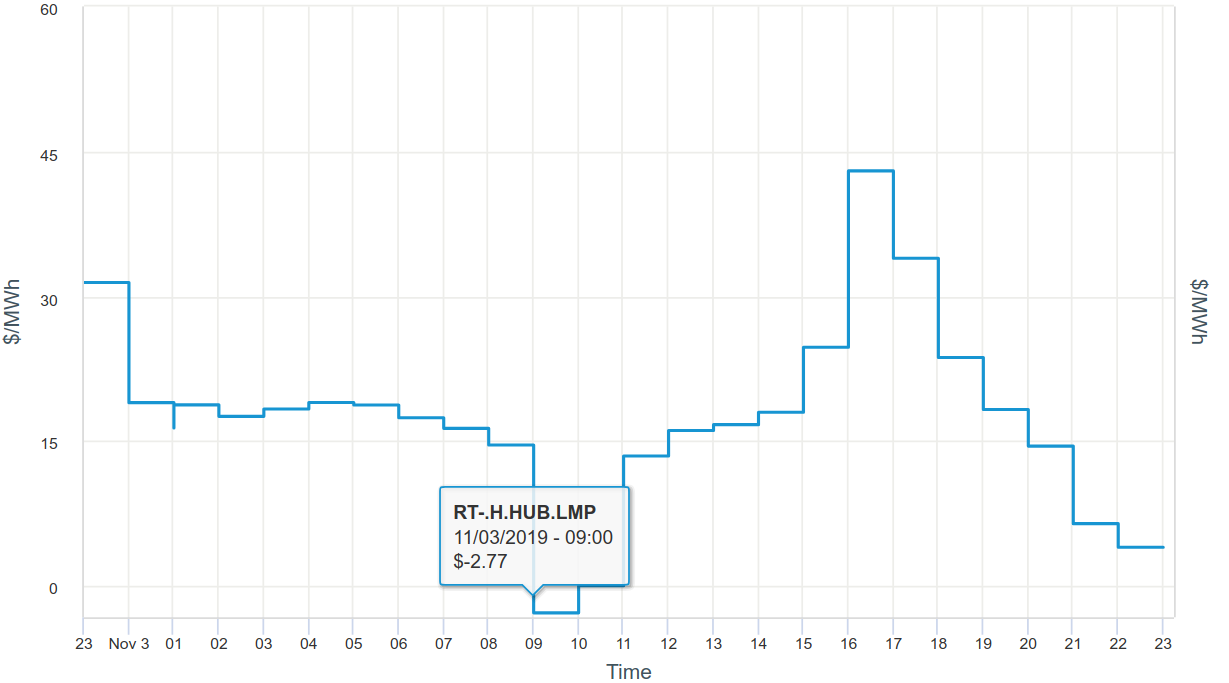
\includegraphics[width=\textwidth]{./images/ne_one_day_price.png}
		\vspace{-6mm}
	\caption{ISO New England hourly electricity price; November 3, 2019 
	from 00:00AM to 11:00PM (Source: https://www.iso-ne.com/).}
\end{figure}  
\end{textblock*}
\end{frame}

\begin{frame}
\frametitle{Nuclear Power Plant Load-Following}
        \begin{block}{Limitations to \gls{LWR} power maneuvering \cite{lokhov_technical_2011}}
	\begin{enumerate}
		\item<1-> Thermal strain and stress to fuel materials.
		\item<1-> Moderator effect (primary coolant temperature change)
		\item<1-> Doppler effect (fuel temperature change)
		\item<1-> Fuel burnup (low excess reactivity at the end-of-cycle 
		(EOC))
        \item<3-> \textbf{$^{135}Xe$ poisoning (iodine pit)}
	\end{enumerate}
\end{block}
\end{frame}

\begin{frame}
\frametitle{What is Xenon-135 poisoning? \cite{noauthor_nuclear_nodate-1}}
\animategraphics[loop,controls,width=1.07\linewidth]{0.5}{./images/anime/xe_pois-}{0}{11}
\end{frame}

\subsection{Molten Salt Reactors}

%\begin{frame}
%\frametitle{Potential Generation IV reactor systems 
%%%\cite{abram_generation-iv_2008}}
%\begin{figure}[t]%
%	\vspace*{-0.1in}
%	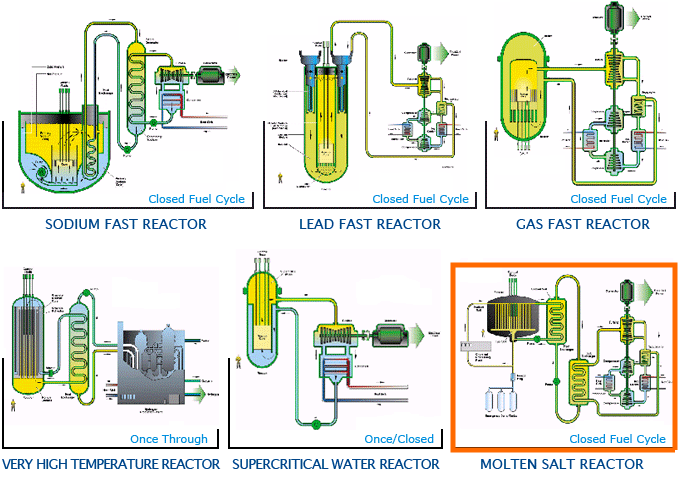
\includegraphics[height=0.7\textwidth]{./images/6_types.png}
%	\caption{\gls{MSR} design}
%\end{figure}            
%\end{frame}

\begin{frame}
\frametitle{MSR (Molten Salt Reactor) types}
\begin{textblock*}{12cm}(0.4cm,1.9cm) % {block width} (coords)
\begin{overlayarea}{\linewidth}{20\baselineskip}
\begin{block}{Stationary Fuel}<1->
	\begin{enumerate}
				\item Graphite block with TRISO fuel, clean salt works as 
				coolant (Fluoride-Salt-Cooled High-Temperature Reactor (FHR))
				\item Plate Fuel: hexagonal fuel assembly is similar in shape 
				to a typical sodium-cooled reactor
				\item Fuel Inside Radial Moderator (FIRM)
	\end{enumerate}
\end{block}

\begin{block}{Mobile Fuel}<2->
	\begin{enumerate}
		\item \textbf{Solid}
			\begin{itemize}
				\item<2-> Mobile solid fuel elements (pebbles) cooled by 
				clean salt (PB-FHR)
			\end{itemize}
			\item<3-> \textbf{Liquid}
			\begin{itemize}
				\item<3-> Without on-site fuel reprocessing facility 
				(TerraPower \glsfirst{MCFR})
				\item<4-> \textbf{With on-site fuel reprocessing} 
				(\glsfirst{TAP} MSR, \glsfirst{MSBR})
			\end{itemize}
	\end{enumerate}
\end{block}
\end{overlayarea}
\end{textblock*}
\end{frame}


%\begin{frame}
%\frametitle{Stationary and Mobile Solid fuel}
%\vspace*{-0.1in}
%\begin{figure}[t]
%	\hspace*{-0.35in}
%	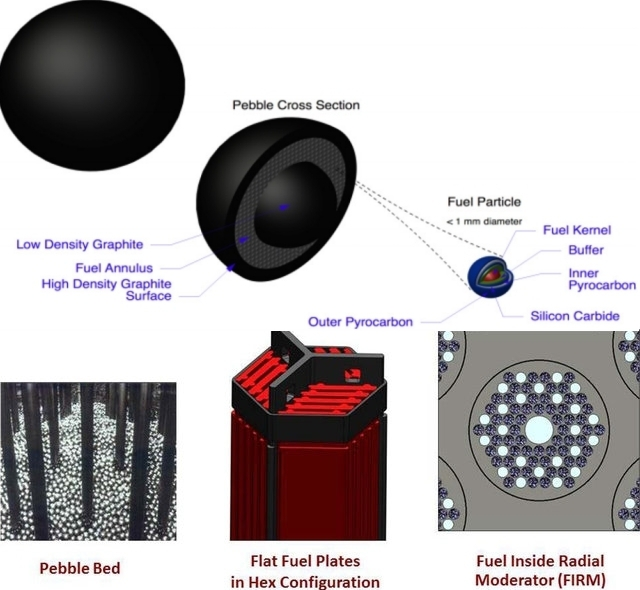
\includegraphics[height=0.63\textwidth]{./images/solid_fuel.jpg}
%	\caption{TRISO fuel particle (top) and FHR fuel designs (bottom) 
%	\cite{forsberg_basis_2016}.} 
%\end{figure}   
%\end{frame}

%\begin{frame}
%\frametitle{Mobile, Non-Circulating, Liquid Fuel}
%\begin{figure}[t]
%\vspace*{-0.1in}
%\hspace*{-0.35in}
%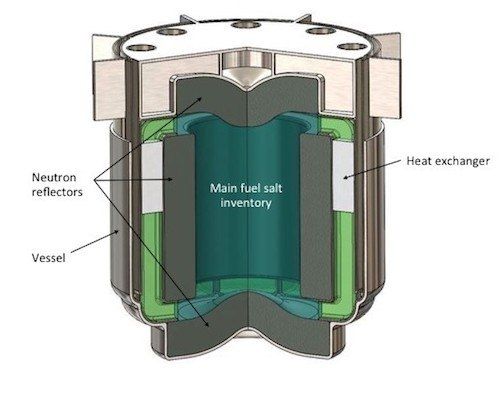
\includegraphics[height=0.6\textwidth]{./images/mcfr-crossection.jpg}
%\caption{The TerraPower MCFR is an example of reactor design with 
%\textbf{liquid, mobile} chloride salt fuel but \textbf{without on-site 
%reprocessing} \cite{doene_southern_2018}.}
%\end{figure}   
%\end{frame}


\begin{frame} % Add another slide with red rectangular around reprocessing system
\frametitle{Mobile, Liquid Fuel with on-site reprocessing facility}
\vspace{-3mm}
\begin{figure}[t]
      \includegraphics[height=0.67\textwidth]{./images/tap_primary_loop.png}
    \vspace{-2mm}
	\caption{The TAP reactor conceptual schematic (including reprocessing 
	system) \cite{transatomic_power_corporation_technical_2016}.}
\end{figure}   

\end{frame}


\subsection{Motivation}

%\begin{frame}
%\frametitle{Why Molten Salt Reactors with circulating fuel?}
%\begin{block}{Liquid-fueled MSR designs have following \textbf{potential} 
%advantages:}
%	\begin{enumerate}
%		\itemsep1em
%		\item High coolant temperature (600-750$^{\circ}$C) 
%		$\Rightarrow$ potentially high thermal efficiency, process 
%		heat for chemical industry
%		\item Fuel diversity ($^{235}$U, $^{233}$U, Thorium, U/Pu)
%		\item Strong negative fuel temperature feedback 
%		\item Passive safety $\Rightarrow$ fuel drains into tanks 
%		in emergency
%		\item High fuel utilization $\Rightarrow$ reduced spent fuel 
%		generation
%		\item<2> \textbf{On-line (continuous) fuel reprocessing potentially  
%		helps to reduce Xenon-135 poisoning} $\Rightarrow$ more flexible  
%		power maneuvering
%	\end{enumerate}
%\end{block}

%\end{frame}


\subsection{Research objectives}

\begin{frame}
  \frametitle{Research objectives of this work}
     Analyze TAP MSR neutronic performance during load-following 
     \textbf{at the \glsfirst{BOL}} and \textbf{without online fission 
     product removal}. The neutronics performance for the Middle of 
     Life and End of Life will be different, and will require fission product 
        removal.
  \begin{overlayarea}{\linewidth}{20\baselineskip}
     \begin{block}{Goals of current study}<1->
         \begin{enumerate}
         		\itemsep1em
                \item<1-> Create high-fidelity full-core 3-D model of 
                TAP concept, without any approximations using Serpent 
                \cite{leppanen_serpent_2014}
                \item<2-> Perform fuel salt depletion to study 
                \textbf{$^{135}$Xe/$^{135}$I balance dynamics during 
                load-following}
            	\item<3-> Analyze $k_{eff}$ dynamics during 
            	\textbf{load-following}
                \item<4-> Compare obtained results with well-studied 
                \glsfirst{PWR} behavior
         \end{enumerate}
      \end{block}
  \end{overlayarea}
\end{frame}

\section{Methodology}
\subsection{Fuel salt reprocessing system}

\begin{frame}
  \frametitle{Fuel salt reprocessing system overview: gas separation}
  Gaseous fission products (e.g., Xe, Kr) must be removed from the fuel salt 
  to avoid reactor
poisoning. 
  
      \begin{columns}
      	\column[t]{4.7cm}
    \begin{block}{Noble gas removal}
      \begin{enumerate}
      	\item bubble generator injects He bubbles in the salt stream
      	\item noble gas migrate to the He bubbles 
      	\item gas separator discharges the poison-rich bubbles
      \end{enumerate}
    \end{block}    	
      	
     	\column[t]{8cm}
  \begin{figure}[t]
	  \centering
	  		\vspace{-8mm}
		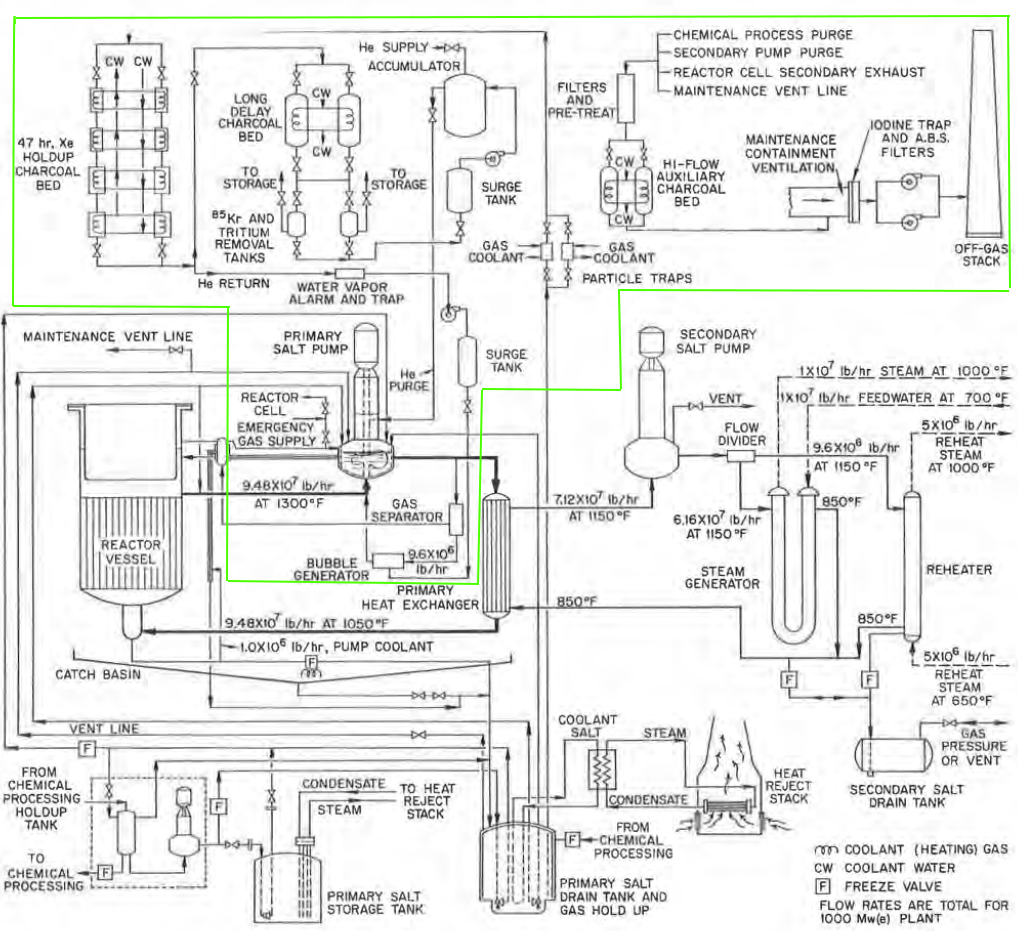
\includegraphics[width=\textwidth]{../figures/gas_separation.pdf}
	\caption{Schematic flow diagram of the \gls{MSBR} gas separation system 
	(figure reproduced from Robertson \emph{et al.}  
	\cite{robertson_conceptual_1971}).} 
    \end{figure}

	\end{columns}
\end{frame}

\begin{frame}
  \frametitle{Mathematical model for gas separation efficiency}
  		\vspace{-1mm}
Xenon removal efficiency ($\epsilon_{Xe}$) in a gas separation system is 
\cite{peebles_removal_1968}:
\begin{align}
& \qquad\qquad \epsilon_{Xe} = \frac{1-e^{-\beta}}{1+\alpha} \nonumber \\
\alpha &= \frac{RTQ_{L}}{HQ_{G}} \nonumber \\
\beta &= \frac{K_L a A_C L (1+\alpha)}{Q_{L}} \nonumber \\
Q_{L}&= \mbox{volumetric salt flow rate} \nonumber \\
Q_{G}&= \mbox{volumetric helium flow rate} \nonumber \\
H &= \mbox{Henry's law constant} \nonumber \\
a &= \mbox{gas-liquid interfacial area} \nonumber \\
K_L &= \mbox{liquid phase mass transfer coefficient.} \nonumber
\end{align}
		\vspace{-5mm}
  \begin{figure}[t]
	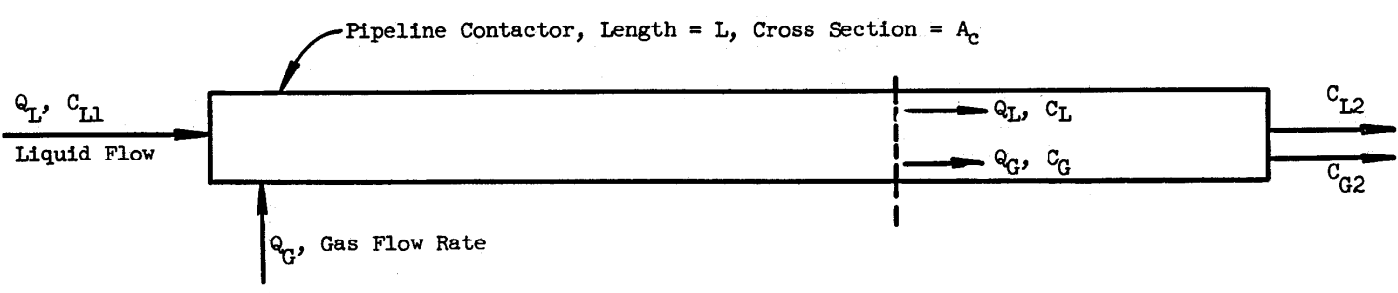
\includegraphics[width=0.66\textwidth]{./images/pipeline_contactor.png}
	\vspace{-2mm}
	\caption{Flow diagram for gas separator (figure reproduced from Peebles 
		\emph{et al.} \cite{peebles_removal_1968}).}
\end{figure}

\end{frame}


\begin{frame}
\frametitle{Fuel processing system overview: rare earths and Pa removal}
	\begin{figure}[htp!] % replace 't' with 'b' to 
		\centering
			\includegraphics[width=0.57\textwidth]{../figures/flowsheet.pdf}
			\vspace{-2mm}
		\caption{Liquid metal (Bi) extraction system for the \gls{MSBR} 
		(reproduced from Sorensen \cite{sorensen_one-fluid_2006}).} 
	\end{figure}
	
\end{frame}


\begin{frame}
\frametitle{Fuel processing system overview: TAP concept}
	\vspace{-2mm}
\begin{figure}[htp!] % replace 't' with 'b' to 
	\centering
	\includegraphics[width=0.75\textwidth]{../figures/tap_primary_loop.png}
	\caption{Simplified \gls{TAP} primary loop design including off-gas system 
		(blue), nickel filter (orange) and liquid metal extraction system 
		(green) \cite{transatomic_power_transatomic_2019}.}
\end{figure}

\end{frame}


\begin{frame}
\frametitle{SaltProc demonstration for TAP concept input data}
	  \begin{textblock*}{12.5cm}(0.5cm,1.5cm) % {block width} (coords)
%%%%%%%%%%%%%%%%%%%%%%%%%%%%%%%%%%%%%%%%
\begin{table}[htbp!]
	\fontsize{6}{9}\selectfont
	\centering
	\caption{The effective cycle times for fission products removal  from the 
		\gls{TAP} reactor \cite{betzler_implementation_2017}.}
	\begin{tabular}{p{0.14\textwidth} p{0.3\textwidth} p{0.11\textwidth} 
			p{0.11\textwidth}}
		\hline 
		\textbf{Processing group} & \qquad\qquad\qquad \textbf{Nuclides} & 
		\textbf{Removal Rate (s$^{-1}$)} & \textbf{Cycle time (at full power)} 
		\\ \hline 
		\multicolumn{3}{c}{\textit{Elements removed in \gls{MSBR} concept and 
				adopted for the \gls{TAP}} \cite{robertson_conceptual_1971}} \\
		Noble gases & Xe, Kr								  & 5.00E-2 & 20 
		sec \\
		Noble metals & Se, Nb, Mo, Tc, Ru, Rh, Pd, Ag, Sb, Te & 5.00E-2 & 20 
		sec \\
		Seminoble metals & Zr, Cd, In, Sn	  				  & 5.79E-8 & 200 
		days\\
		Volatile fluorides & Br, I 							  & 1.93E-7 & 60 
		days\\
		Rare earths & Y, La, Ce, Pr, Nd, Pm, Sm, Gd           & 2.31E-7 & 50 
		days\\
		\qquad & Eu & 2.32E-8 & 500 days \\
		Discard & Rb, Sr, Cs, Ba & 3.37E-9 & 3435 days \\
		\hline
		\multicolumn{3}{c}{\textit{Additional elements removed} 
			\cite{betzler_implementation_2017, 
			transatomic_power_corporation_neutronics_2016}} \\
		Noble gases & H								  	& 5.00E-2 & 20 
		sec    \\
		Noble metals & Ti, V, Cr, Cu						& 3.37E-9 & 3435 
		days \\
		Seminoble metals & Mn, Fe, Co, Ni, Zn, Ga, Ge, As   & 3.37E-9 & 3435 
		days \\
		Rare earths & Sc									& 3.37E-9 & 3435 
		days \\
		Discard & Ca										& 3.37E-9 & 3435 
		days \\
		\hline
	\end{tabular}
	\label{tab:reprocessing_list}
\end{table}
	\begin{itemize}
		\item Noble gas removal efficiency: variable, described using 
		mathematical 
		correlation
		\item Other FP removal efficiency: fixed, non-ideal, based on 
		Table~\ref{tab:reprocessing_list}
	\end{itemize}
	\end{textblock*}
\end{frame}


\subsection{Proposed tool design}


\begin{frame}
\frametitle{SaltProc class architecture}
	\begin{itemize}
		\item \textit{Simulation} class
			\begin{itemize}
				\item Manages simulation process
				\item Stores data into the HDF5 database
				\item Tracks time
			\end{itemize}
		\item \textit{Depcode} class
			\begin{itemize}
				\item Contains attributes and methods for reading user's input
				\item Creates input files for depletion code
				\item Parses depletion code output 
			\end{itemize}
		\item \textit{Process} class
			\begin{itemize}
				\item Represents fuel processing system component
				\item Contains attributes of the component ($\epsilon_e$, throughput rate, capacity)
				\item Tracks waste stream
			\end{itemize}
		\item \textit{MaterialFlow} class
			\begin{itemize}
				\item Instances of that class represents the material flowing between processes
			\end{itemize}
	\end{itemize}
		\vspace{3mm}
	\begin{figure}[ht!] % replace 't' with 'b' to 
		\centering
		\includegraphics[width=0.6\textwidth]{../figures/materialflow.pdf}
		\vspace{-0.1in}
		\caption{Schematic for passing material data between fuel processing 
		system components.}
	\end{figure}

\end{frame}


\begin{frame}
\frametitle{SaltProc flowchart}
\vspace{-2mm}
\begin{figure}[ht!] % replace 't' with 'b' to \centering
	\centering
	\includegraphics[width=1.05\textwidth]{./images/saltproc_flowchart.pdf}
	\caption{Tentative generic flowchart for SaltProc v1.0 python package.}
\end{figure}

\end{frame}
\section{Results}
\subsection{Multiplication factor dynamics}

\begin{frame}
\frametitle{Multiplication factor dynamics after shutdown}
\begin{textblock*}{12.5cm}(0.2cm,1.5cm) % {block width} (coords)
\begin{columns}
	\column[t]{6cm}
	\begin{figure}[t]
		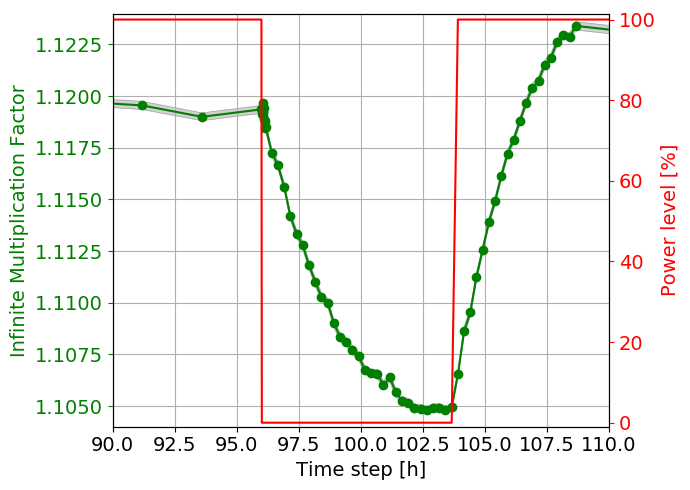
\includegraphics[width=\linewidth]{./images/pwr_keff_zoomed.png}
		\vspace{-6mm}
		\caption{Multiplication factor for PWR assembly after 
		shutdown ($\sigma\pm20$pcm shaded).}
	\end{figure}
		\vspace{-5mm}
	\begin{enumerate}             
		\item $-1500pcm$ reactivity insertion due to $^{135}$Xe poisoning
		\item $k_{\infty}$ reached local minima $\approx7$ hrs after shutdown
		\item overall reactivity swing $1750pcm$
	\end{enumerate}

	\column[t]{6cm}
	\visible<2->{

		\begin{figure}[t]
		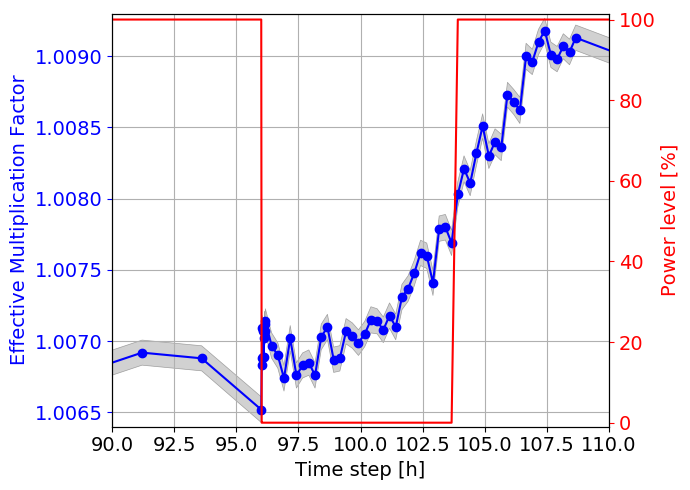
\includegraphics[width=\linewidth]{./images/tap_keff_zoomed.png}
		\vspace{-6mm}
		\caption{Multiplication factor for
TAP after 
			shutdown ($\sigma\pm7.5$pcm shaded).}
		\end{figure}
		\vspace{-5mm}
		\begin{enumerate}             
		\item $+130pcm$ reactivity insertion because loss of $^{135}$Xe from  
		decaying to $^{135}$Cs is larger than gain from $^{135}$I decay
		\item $k_{\infty}$ has no local minima
		\item overall reactivity swing $270pcm$
		\end{enumerate}

	}

\end{columns}
\end{textblock*}
\end{frame}

\subsection{$^{135}$Xe/$^{135}$I balance}
\begin{frame}
\frametitle{Fuel salt composition dynamics}
\begin{textblock*}{12.5cm}(0.2cm,2cm) % {block width} (coords)
	\begin{columns}[t,onlytextwidth]
		\column{.5\textwidth}
		\begin{figure}[t]
	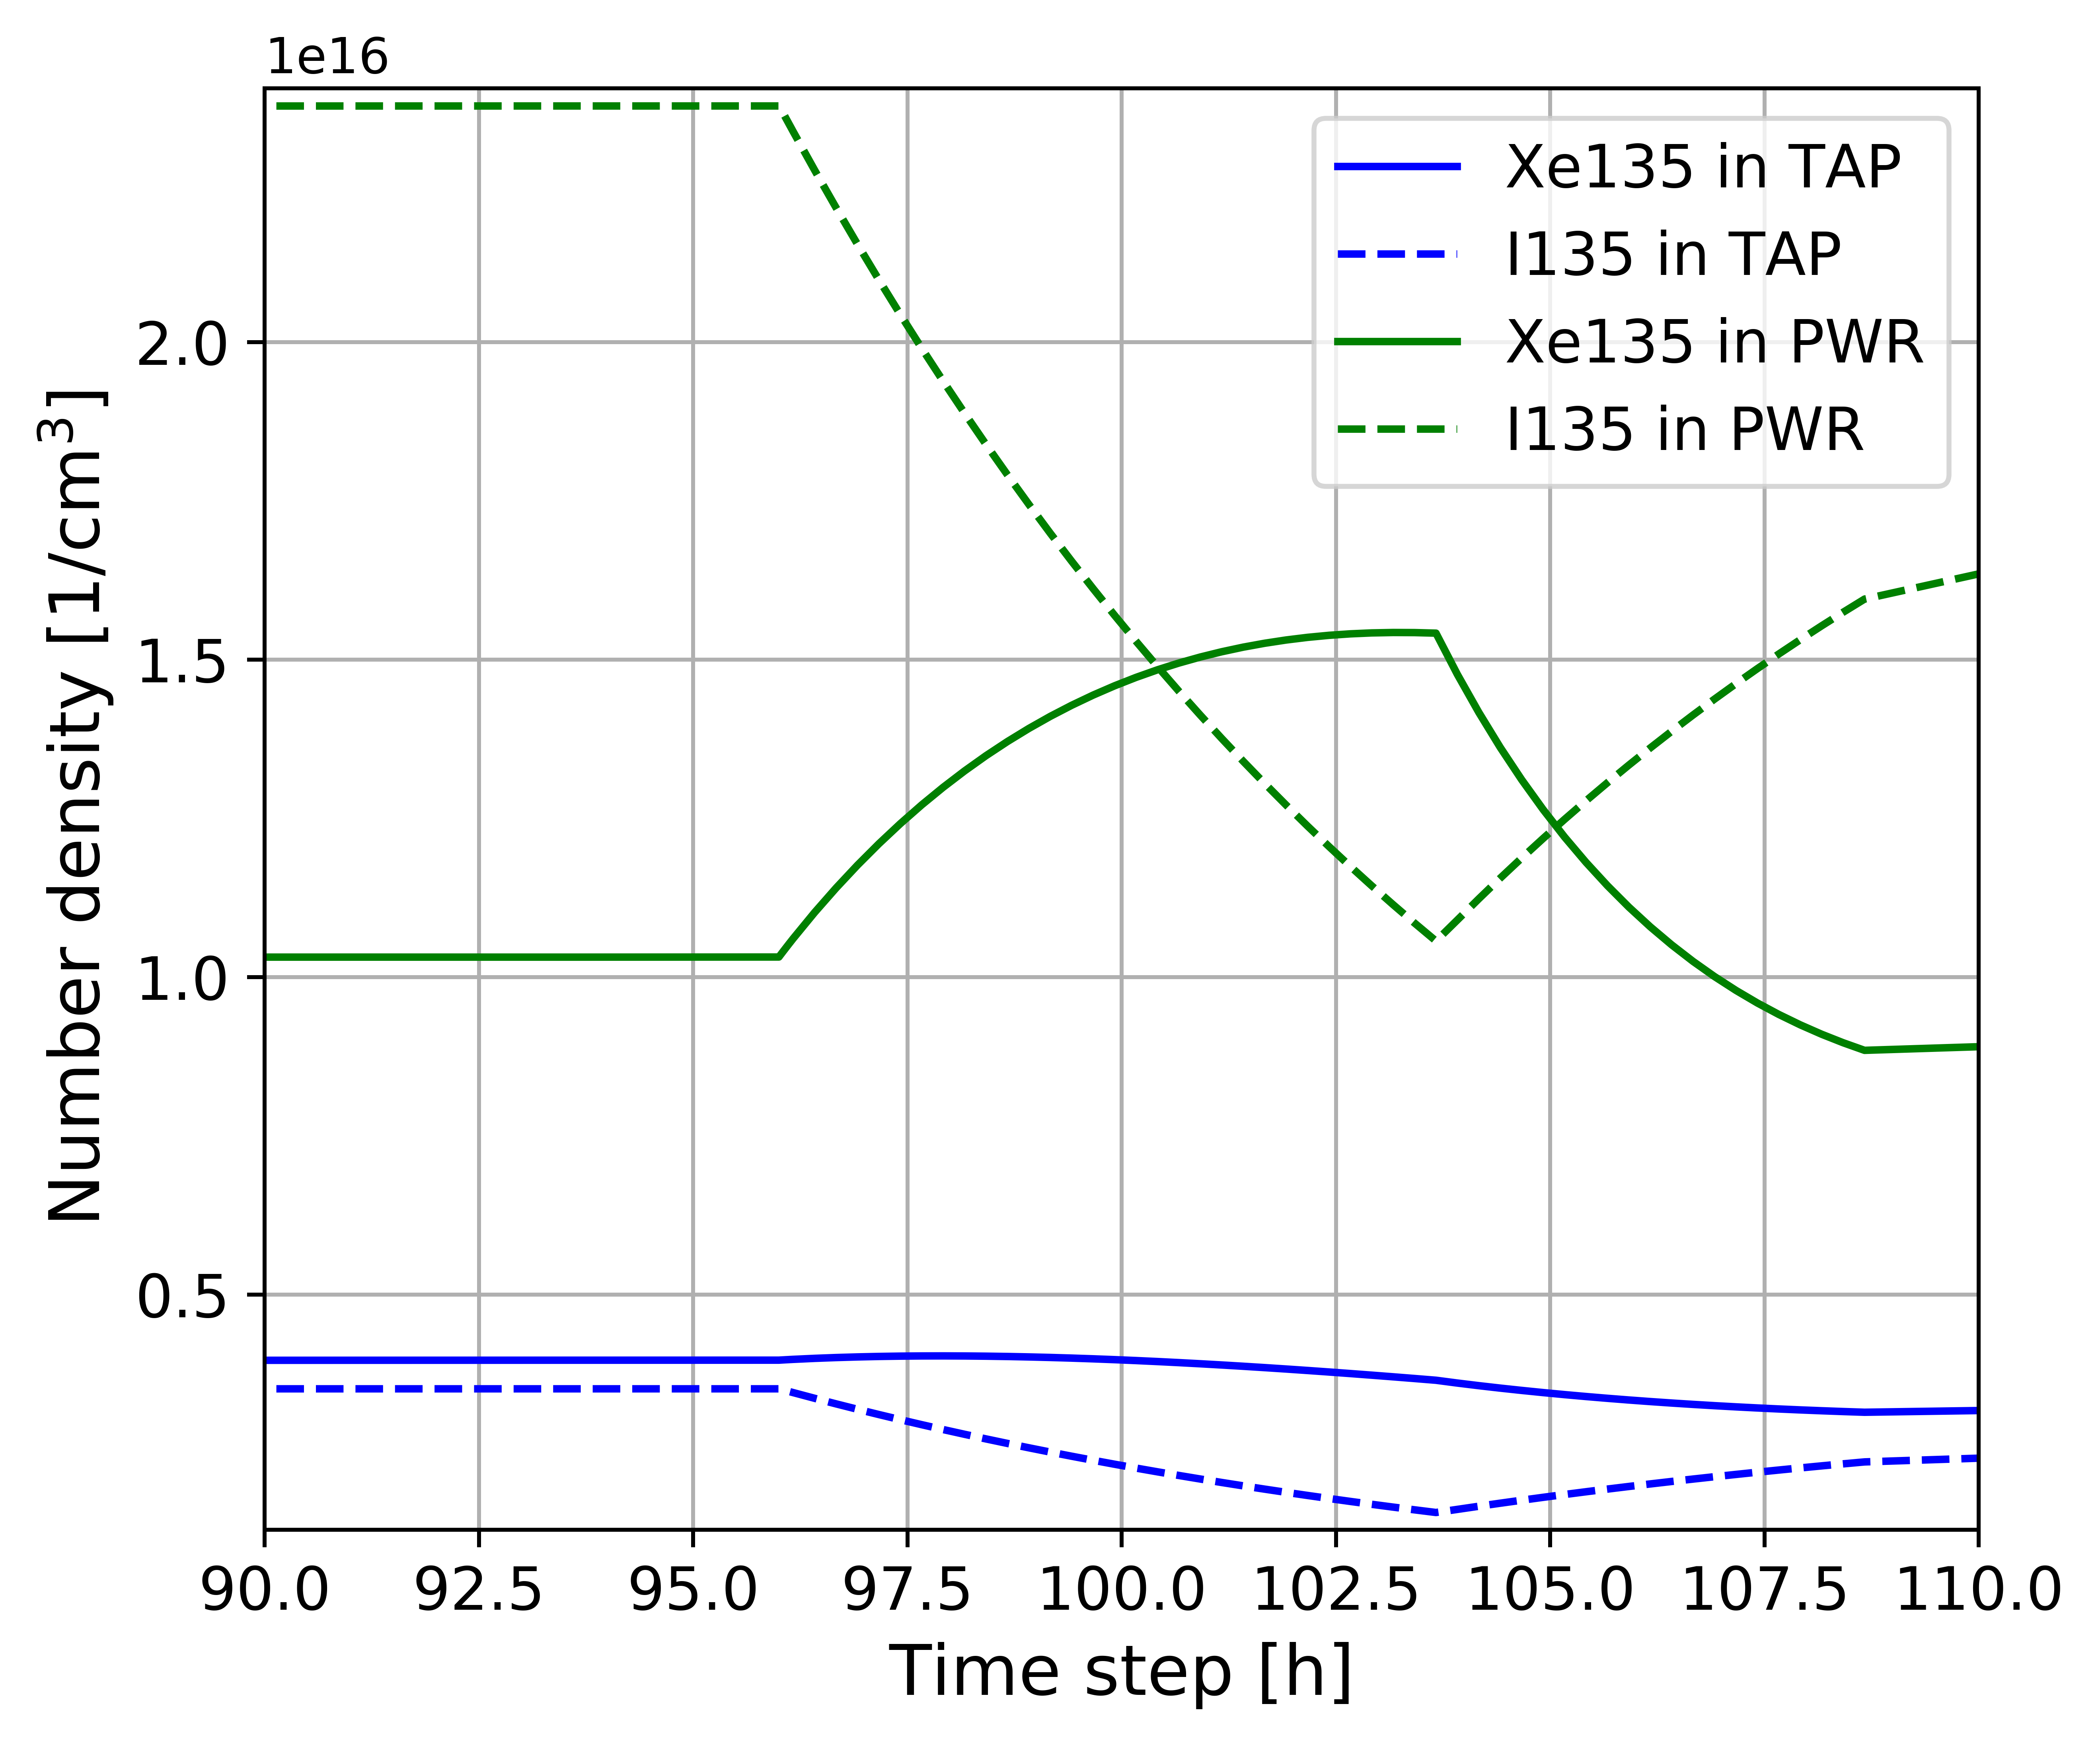
\includegraphics[width=\linewidth]{./images/tap_vs_pwr_xe_i_density.png}
		\caption{Atomic density of $^{135}$Xe and its main precursor 
		($^{135}$I) after shutdown.}
		\end{figure}
		\column{.5\textwidth}
			\vspace{+5mm}
		\begin{block}{Why no poisoning effect?}
			\begin{enumerate}             
				\item $^{135}$I/$^{135}$Xe number density ratio is 2.3 (PWR) 
				and 0.9 (TAP)
				\item $^{135}$I half-life 6.6h $<$ $^{135}$Xe half-life 9.2h
				\item PWR accumulated significant $^{135}$I inventory which 
				caused large xenon concentration  peak ($150\%$)
				\item In TAP, $^{135}$Xe gain from $^{135}$I decay did
				not overcome $^{135}$Xe decay loss
				\item Maybe because the neutron spectrum is different?
			\end{enumerate}
		\end{block}
	\end{columns}
\end{textblock*}
\end{frame}

\subsection{Neutron spectra}

\begin{frame}
\frametitle{Neutron spectra of PWR vs TAP}
\begin{textblock*}{12.3cm}(0.2cm,2cm) % {block width} (coords)
	\begin{columns}[t,onlytextwidth]
		\column{.6\textwidth}
		\begin{figure}[t]
			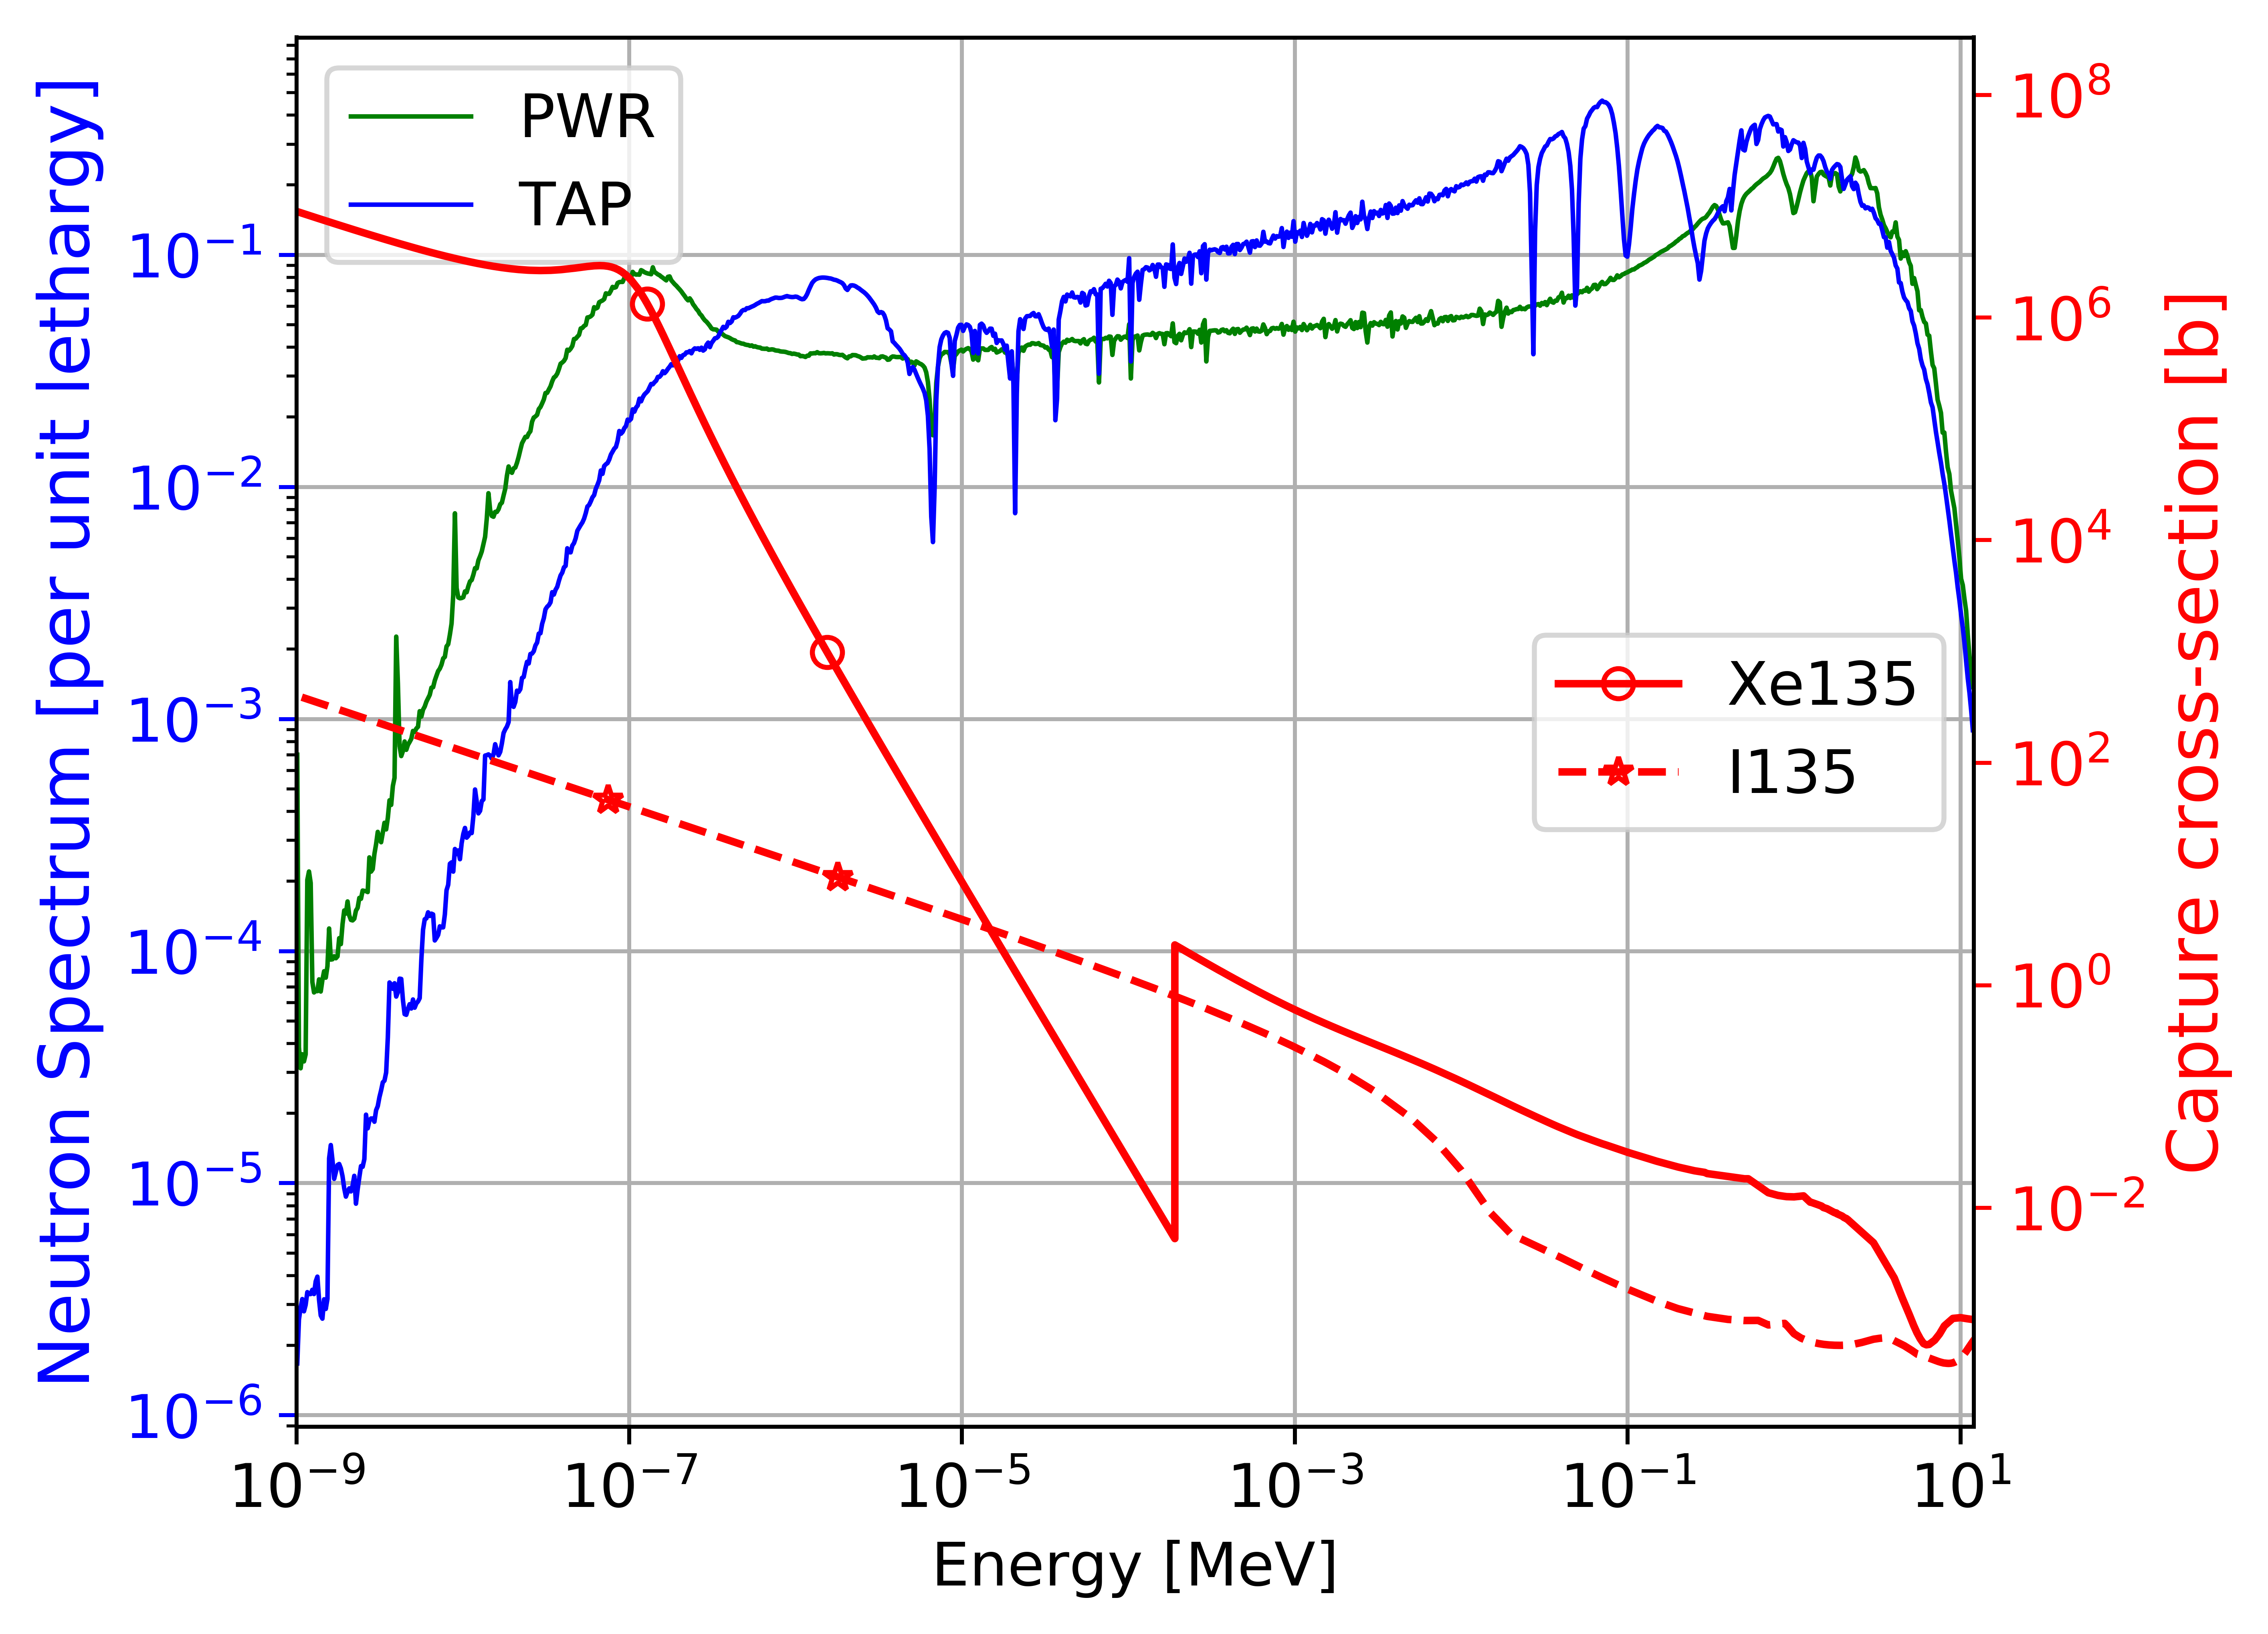
\includegraphics[width=\linewidth]{./images/spectra.png}
			\caption{Neutron spectra normalized by lethargy for the PWR and 
			TAP vs. $^{135}$Xe and $^{135}$I caption cross-section.}
		\end{figure}
	
	
		\column{.4\textwidth}
		\vspace{+1mm}
		\begin{block}{Why different $^{135}$I/$^{135}$Xe balance?}
			\begin{enumerate}             
				\item TAP at beginning-of-life has much harder spectrum than 
				PWR
				\item Harder neutron spectrum leads to weaker $^{135}$Xe 
				transmutation to $^{136}$Xe due to \textbf{strong energy 
				dependence of the capture cross-section}
				\item $\sigma_{(n,c)}$ slope is much steeper  for 
				$^{135}$Xe than for $^{135}$I
			\end{enumerate}
		\end{block}
	\end{columns}
\end{textblock*}
\end{frame}
\section{Conclusions}
\begin{frame}
\frametitle{Completed and future work}       
\begin{textblock*}{12.5cm}(0.1cm,2.2cm) % {block width} (coords)
	\begin{figure}[ht!] % replace 't' with 'b' to force it to 
		\includegraphics[width=\textwidth]{./images/progress_chart_larger.pdf} 
	\end{figure}
\end{textblock*}
\end{frame}

\begin{frame}
\frametitle{Conclusion}
	\begin{textblock*}{12cm}(0.4cm,2cm) % {block width} (coords)
	\begin{itemize}
		\itemsep1em
		\item Relevance
		\begin{itemize}
			\itemsep0.5em
			\item Fuel salt processing systems modeling in \glspl{MSR} based 
			on \textbf{many assumptions and estimations}
			\item This work will \textbf{more realistically} model salt 
			processing system with a \textbf{focus on the gas removal system}  
			of the prospective \gls{TAP} \gls{MSR}
		\end{itemize} 
		\item Preliminary results
			\begin{itemize}
				\itemsep0.5em
				\item Simple demonstration for \gls{MSBR} with 
				\textbf{ideal/fixed	fission products removal efficiency}
				\item \textbf{Multi-component} fuel reprocessing system 
				modeling with \textbf{non-ideal/constant} 
				efficiency
				\item \textbf{Effect of fission product removal} on the core 
				neutronics
			\end{itemize}
		
		\item Future work
			\begin{itemize}
				\itemsep0.5em
				\item Add \textbf{variable geometry} and \textbf{dynamic 
				removal efficiency capability}
				\item Demonstrate and validate those capabilities for 
				\textbf{lifetime-long depletion}
				\item Simulate short-term transients to determine the 
				\textbf{feasibility of load following}
				\item Determine feasible \textbf{design parameters of the 
				sparger}
				\item Analyze \textbf{dynamics of the safety parameters} for 
				long- and short-term cases
			\end{itemize}
	\end{itemize}
\end{textblock*}
\end{frame}

\begin{frame}
	\frametitle{Questions?}
\end{frame}
%%--------------------------------%%
%%--------------------------------%%
\begin{frame}[allowframebreaks]
  \frametitle{References}
  \bibliographystyle{unsrt}
  {\footnotesize \bibliography{../2019-rykhl-xenon-ans} }

\end{frame}

%%--------------------------------%%
%%---BACKUP SLIDES----------------%%


\end{document}



